\documentclass{article}
% This is a LaTeX file.  It is a text file that is compiled
% by a program called LaTeX into a pretty PDF file.  
% If you're viewing this file on CoCalc, you'll see that PDF 
% in the window to the right.
%
% The LaTeX macro language is complicated, so we have inserted
% lots of documenting comments into the file.  Comments start
% with `%' and continue to the end of the line.  In CoCalc's
% window, they are colored brownish-red.
%
% Comments prefixed with `Student:' are relevant to students.
% Skip anything else you don't understand, or ask me.
%
% set font encoding for PDFLaTeX or XeLaTeX
\usepackage{ifxetex}
\ifxetex
  \usepackage{fontspec}
\else
  \usepackage[T1]{fontenc}
  \usepackage[utf8]{inputenc}
  \usepackage{lmodern}
\fi

% Student: These lines describe some document metadata.
\title{Problem Set 3}
\author{%
% Student: change the next line to your name!
    Name
\\  MATH-UA 120 Discrete Mathematics
}
\date{due February 17, 2023}


\usepackage[headings=runin-fixed-nr]{exsheets}
% These make enumerates within questions start at the second ("(a)") level, rather than the first ("1.") level.
\makeatletter
    \newcommand{\stepenumdepth}{\advance\@enumdepth\@ne}
\makeatother
\SetupExSheets{
    question/pre-body-hook=\stepenumdepth,
    solution/pre-body-hook=\stepenumdepth,
}
\DeclareInstance{exsheets-heading}{runin-nn-np}{default}{
    runin = true,
    title-post-code = .\space,
    join = {
        main[r,vc]title[l,vc](0pt,0pt);
    }
}
\newif\ifshowsolutions
% Student: replace `false' with `true' to typeset your solutions.
% Otherwise they are ignored!
\showsolutionstrue
\ifshowsolutions
    \SetupExSheets{
        question/pre-hook=\itshape,
        solution/headings=runin-nn-np,
        solution/print=true,
        solution/name=Answer
    }%
    \makeatletter%
    \pretocmd{\@title}{Answers to }%
    \makeatother%
\else
    \SetupExSheets{solution/print=false}
\fi

% Bug workaround: http://tex.stackexchange.com/a/146536/1402
%\newenvironment{exercise}{}{}
\RenewQuSolPair{question}{solution}
%\let\answer\solution
%\let\endanswer\endsolution
\usepackage{manfnt}
\newcommand{\danger}{\marginpar[\hfill\dbend]{\dbend\hfill}}

\usepackage{subcaption}

\newcommand{\Z}{\mathbb{Z}}
\newcommand{\R}{\mathbb{R}}
\newcommand{\N}{\mathbb{N}}
\newcommand{\Q}{\mathbb{Q}}

\usepackage{amsmath, amsthm}
\usepackage{amsfonts}
\usepackage{enumerate}
\usepackage{siunitx}
\DeclareSIUnit\pound{lb}
\usepackage{hyperref}
\newtheorem*{theorem}{Theorem}
\newtheorem*{proposition}{Proposition}
\newtheorem*{claim}{Claim}
\theoremstyle{definition}
\newtheorem*{definition}{Definition}
% This is the beginning of the part of the file that describes
% the text of the document.
% That's why it says `\begin{document}' below. :-)
\begin{document}
\maketitle



These are to be written up and turned in to Gradescope.\\



\ifshowsolutions
    \SetupExSheets{solution/print=true}
\else
    \danger
 \underline{ \LaTeX  Instructions:}  You can view the source (\texttt{.tex}) file to get some more examples of \LaTeX{} code.  I have commented the source file in places where new \LaTeX{} constructions are used.
  
  Remember to change \verb|\showsolutionsfalse| to \verb|\showsolutionstrue|
    in the document's preamble 
    (between \verb|\documentclass{article}| and \verb|\begin{document}|)
\fi

\section*{Assigned Problems}

\begin{question}
   \begin{enumerate}
   \item Consider the following subsets of $\N$.
       \begin{align*}
           A &= \text{The set of all even numbers.}\\
           B &= \text{The set of all prime numbers.}\\
           C &= \text{The set of all perfect squares.}\\
           D &= \text{The set of all multiples of 10.}
       \end{align*}
       Using \textbf{only} the symbols $3, A, B, C, D, \N, \in, \subseteq, =, \neq, \cap, \cup, \times, -, \emptyset$, ``('', and  ``)'', rewrite the following statements in set notation. 
           \begin{enumerate}
               \item None of the perfect squares are prime numbers. 
               \item The number 3 is a prime number that is not even.
               \item If you take all the prime numbers, all the even numbers, all the perfect squares, and all the multiples of 10, you still won't have all the natural numbers.
           \end{enumerate}
   
   \item Consider the following subsets of the set of all students at some university. 
       \begin{align*}
           F &= \text{The set of all freshmen.}\\
           S &= \text{The set of all seniors.}\\
           M &= \text{The set of all math majors.}\\
           C &= \text{The set of all CS majors.}
       \end{align*}
           \begin{enumerate}
               \item Using only the symbols $F, S, M, C, | ~ |, \cap, \cup, -$, and $>$, translate the following statement into the language of set theory. 
               \begin{quote}
                   ``There are more freshmen who aren't math majors than there are senior CS majors.''
               \end{quote}
               \item Translate the following statement in set theory into everyday English. 
               $$(F\cap M)\subseteq C$$
           \end{enumerate}
   \end{enumerate}
\end{question}
% Student: put your answer between the next two lines.
\begin{solution}
\begin{enumerate}
\item 
    \begin{enumerate}
    \item $B\cap C = \emptyset$
    \item $3\in B- A$
    \item $\N -(A\cup B\cup C\cup D) \neq \emptyset$
    \end{enumerate}
\item 
    \begin{enumerate}
    \item $|F - M| > |S\cap C|$
    \item All freshmen math majors double major in CS.
    \end{enumerate}
\end{enumerate}
%%{\color{red} Rubric:
%%\begin{itemize}
%%\item 2P each
%%\end{itemize}}
\end{solution}

\begin{question}
Describe explicitly in English the following sets, then give their cardinality.

\begin{enumerate}
	\item $\{x \in 2^{\Z} : 5 \in x \}$
	\item $\{x \in 2^{\Z} : x \subseteq \{ 1, 2, 3\} \}$
	\item $\{x \in 2^{\Z} : x \subseteq \{ 1, 2, \{3, 4\} \} \}$
	\item $\{x \in 2^{\Z} : x \in \{ 1, 2, \{3, 4\} \} \}$
	\item $\{x \in 2^{\Z} : y \in x \implies y = 0 \}$
\end{enumerate}
\end{question}
% Student: put your answer between the next two lines.
\begin{solution}
\begin{enumerate}
	\item This is the set of all subsets of $\Z$ that contain $5$. There are infinitely many such subsets, like $\{5\}, \{5,6\}, \{5,6, 7\}, \dots$, so $\left | \{x \in 2^{\Z} : 5 \in x \} \right |$ is infinite.
	\item This is the set of all subsets of $\Z$ that are also subsets of $\{1, 2, 3\}$, so it is actually the set of all subsets of $\{1,2,3\}$. Therefore
	\[
	\left |\{x \in 2^{\Z} : x \subseteq \{ 1, 2, 3\} \} \right | = \left | 2^{\{1, 2, 3\}} \right | = 2^{|\{ 1, 2, 3\}|} = 2^3 = 8.
	\]
	
	\item This is the set of all subsets of $\Z$ that are also subsets of $ \{ 1, 2, \{3, 4\} \} \}$. But $\{ 3, 4 \}$ is not an element of $\Z$, so it means that set in question is the set of all subsets of $\{1,2\}$. Therefore, as above, 
	\[
	\left |\{x \in 2^{\Z} : x \subseteq \{ 1, 2, \{3, 4\} \} \} \right | = 2^{|\{1,2 \}|} = 2^2 = 4.
	\]
	
	\item This is the set of all subsets of $\Z$ that are also elements of $ \{ 1, 2, \{3, 4\} \} \}$. But out of these elements, there is only one subset of $\Z$, namely $\{ 3, 4 \}$, and therefore the set in question is the set $\{ \{3,4\} \}$, which contains the one element $\{3,4\}$. Therefore
	\[
	\left | \{x \in 2^{\Z} : x \in \{ 1, 2, \{3, 4\} \} \} \right | = 1.
	\]
	
	\item This is the set of all subsets of $\Z$ such that if there is an element in the subset, then it is $0$. In other words, such a subset can only contain the element $0$, so it is $\{ 0 \}$... or $\emptyset$! Therefore, the set in question is $\{ \emptyset, \{0\}\}$, and thus
	\[
	\left | \{x \in 2^{\Z} : y \in x \implies y = 0 \} \right | = 2.
	\]
\end{enumerate}
%%{\color{red} Rubric:
%%\begin{itemize}
%%\item 2P for each part
%%\item Grader: Please expand on rubric yourself.
%%\end{itemize}}
\end{solution}


\begin{question}
\begin{enumerate}
	\item For each of the following statements, describe it in English, and say if it is true or false (without proof). Then write its negation using quantifier, and express this negation in English. For instance, the statement $\forall x \in \Z \; x < 0$ means every integer is negative, and it is false. Its negation is $\exists x \in \Z \; x \geq 0$, which means that there exists a nonnegative integer.
	
	\begin{enumerate}
		\item $\forall x \in \Z \; \exists y \in \Z \; x^2 + y = 4$
		\item $\exists y \in \Z \; \forall y \in \Z \; x^2 + y = 4$
		\item $\forall n \in \Z \; \exists k \in \Z \; \exists d \in \Z \; k+ n = 2d$
		\item $\exists n \in \Z \; \forall k \in \Z \; \exists d \in \Z \; k+ n = 2d$
	\end{enumerate}
	
	\item For each of the statements (iii) and (iv): prove it if it is true, or prove the negation if it is false. These proofs are short.
\end{enumerate}
\end{question}
% Student: put your answer between the next two lines.
\begin{solution}
\begin{enumerate}
	\item 
	\begin{enumerate}
		\item The statement means to any integer squared, we can add another integer to get 4. This is true. Its negation is
		\[
		\exists x \in \Z \; \forall y \in \Z \; x^2 + y \neq 4
		\]
		which means that we can find an integer squared such that, regardless of what other integer we add to it, we never get a sum equal to 4. 
		
		\item The statement means we can find an integer and add any other integer squared whose sum is 4. This is false. Its negation is
		\[
		\forall y \in \Z \; \exists x \in \Z \; x^2 + y \neq 4
		\]
		which means to any integer, we can add another integer squared and we never get a sum equal to 4.
		
		
		\item The statement means that to any integer, we can add another integer to get an even number. This is true. Its negation is
		\[
		\exists n \in \Z \; \forall k \in \Z \; \forall d \in \Z \; k + n \neq 2d.
		\]
		which means that we can find an integer such that, regardless of what other integer we add to it, we will never get an  even sum.
		
		\item The statement means that there exists an integer such that, regardless of what other integer we add to it, we always get an even sum. This is false. Its negation is
		\[
		\forall n \in \Z \; \exists k \in \Z \; \forall d \in \Z \; k + n \neq 2d.
		\]
		which means that to any integer, we can add another integer and get a sum which is not even.
		
	\end{enumerate}
	\item \begin{itemize}
		\item For part (c): Let us show that
		\[
		\forall n \in \Z \; \exists k \in \Z \; \exists d \in \Z \; k + n = 2d
		\]
		Let $n \in \Z$. Take $k = n$ and $d = n$. Then $k+n = n + n = 2n = 2d$.
		
		\item For part (d): Let us show that
		\[
		\forall n \in \Z \; \exists k \in \Z \; \forall d \in \Z \; k + n \neq 2d
		\]
		Let $n \in \Z$. Take $k = n + 1$. Then $k + n = n+1+n = 2n + 1$ is odd, so it is not even, that is, it cannot be written as $2d$ for any $d \in \Z$.
		
	\end{itemize}
	
\end{enumerate}

%%{\color{red} Rubric:
%%\begin{itemize}
%%\item Part a: 1.5P for each part
%%\item Part b: 2P for each part
%%\item Grader: Please expand on rubric yourself.
%%\end{itemize}}
\end{solution}



\begin{question}
   Let $I=\{1, 2, \dots, n\}$. Given a collection of sets $\{A_1,A_2,\dots, A_n\}$, denoted by $\{A_i\}_{i\in I}$. $\{A_i\}_{i\in I}$ is said to be \textbf{disjoint} if $\cap_{i\in I}A_i=\emptyset$, and it is said to be \textbf{pairwise disjoint} if $A_i\cap A_j=\emptyset$ whenever $i\neq j$. What is the difference between a \textbf{disjoint} collection of sets and a \textbf{pairwise disjoint} collection of sets? (\textit{Draw a picture to convince yourself. You do not need to submit this picture.}) Give an example of a collection of sets that is disjoint, but not pairwise disjoint. (\textit{Hint: You need a minimum of three sets.})
\end{question}
% Student: put your answer between the next two lines.
\begin{solution}
A collection of sets is \textbf{disjoint} if there is no element shared by all sets in the collection; whereas, a collection of sets is \textbf{pairwise disjoint} if no two sets (that are different) share a common element. For example, in the following diagrams, the first picture is disjoint, but not pairwise disjoint and the second picture is pairwise disjoint.
\begin{figure}[h]
\centering
	\begin{subfigure}[h]{.35\textwidth}
	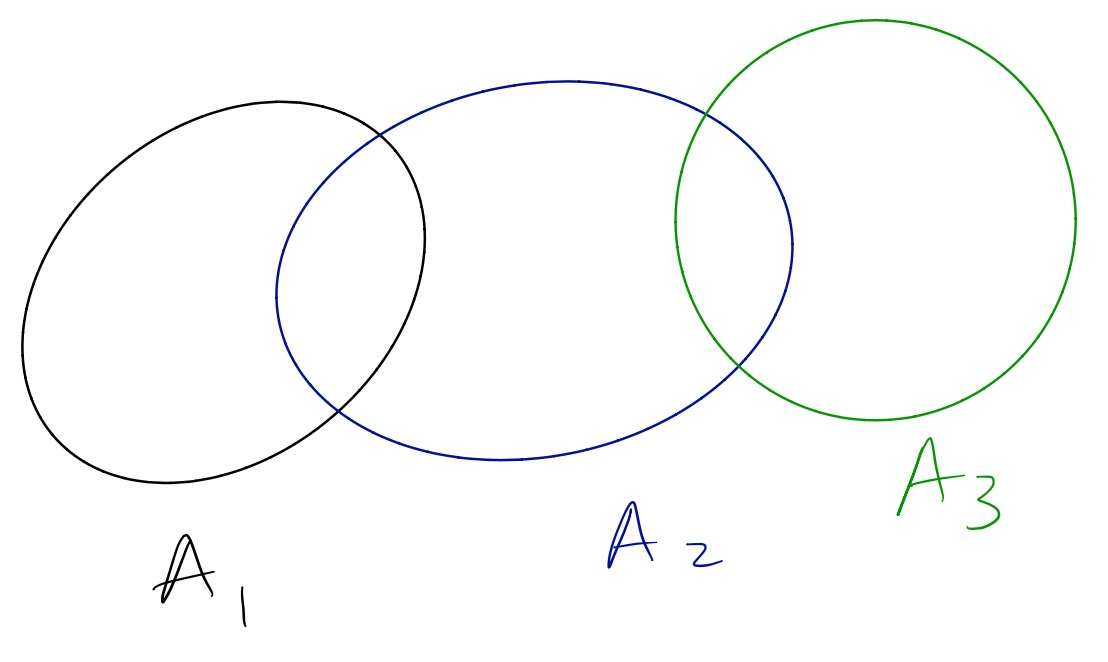
\includegraphics[width=\textwidth]{disjoint}
	\caption{Disjoint but not pairwise disjoint}
	\end{subfigure}
	~\quad\hspace{1cm}
	\begin{subfigure}[h]{.35\textwidth}
	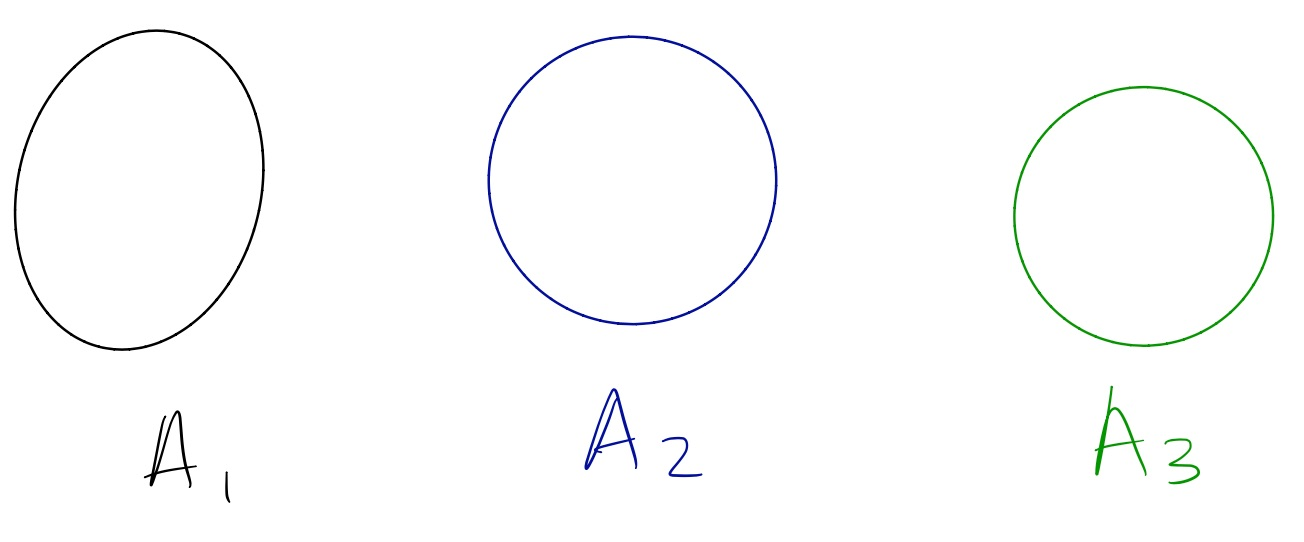
\includegraphics[width=\textwidth]{pair-disjoint}
	\caption{Pairwise disjoint}
	\end{subfigure}	
\end{figure}


\textbf{Example:} Let $A_1=\{1, 2, 3, 4\}, A_2=\{3, 4, 5, 6\}$ and $A_3=\{1, 6, 7\}$.
\begin{itemize}
\item Notice that 
\begin{align*}
A_1\cap A_2\cap A_3 &= (A_1\cap A_2)\cap A_3\\
&=\{3,4\}\cap A_3\\
&=\emptyset.
\end{align*} Hence they are disjoint.
\item However,
\begin{align*}
A_1\cap A_2 &=\{3, 4\}\\
A_1\cap A_3 &=\{1\}\\
A_2\cap A_3 &=\{6\},
\end{align*}
which is not pairwise disjoint.
\end{itemize}

%%{\color{red} Rubric:
%%\begin{itemize}
%%\item 5P for explanation
%%\item 5P for example and explanation of example.
%%\end{itemize}}
\end{solution}


\begin{question}
   Let $E$ be the set of all even integers and let $O$ be the set of all odd integers. Let $X=\{ n\in \Z : n = x+y \text{ for some } x, y\in O\}$. Prove $X=E$.
\end{question}
% Student: put your answer between the next two lines.
\begin{solution}
\begin{proof}
We will prove $X=E$, by first proving $X \subseteq E$ and then $E\subseteq X$.
\begin{enumerate}
\item[($\subseteq$)] Suppose $n\in X$. By definition, there exists $x, y \in O$ such that $n= x+y$. Since $x, y\in O$, there exist $a, b\in Z$ such that $x=2a+1$ and $y=2b+1$. Then
\begin{align*}
n &= x+ y \\
&= (2a+1) + (2b+1)\\
& = 2(a+b+1).
\end{align*}
Thus $2 \mid n$, which implies that $n\in E$. We have $X\subseteq E$.

\item [($\supseteq$)] Suppose $n\in E$. By definition, $2 \mid n$; meaning, there exists $a\in \Z$ such that $n=2a$. Let $b\in \Z$. Observe
\begin{align*}
n &= 2a\\
&= 2a + 2b - 2b + 1 -1 + 1 -1\\
& = (2a - 2b +1) + (2b -1 -1 + 1)\\
& = 2(a-b) + 1 + 2(b-1) + 1.
\end{align*}
Note $2(a-b) + 1$ and  $2(b-1) + 1$ are some odd integers. We have $E\subseteq X$.
\end{enumerate}
Therefore, $X=E$.
\end{proof}
%%{\color{red} Rubric:
%%\begin{itemize}
%%\item Follow RVF rubric with 1P for \LaTeX
%%\end{itemize}}
\end{solution}

\end{document}


